\documentclass[a4paper,11pt,twoside]{article}
\usepackage{amssymb}
\usepackage{hyperref}
\usepackage{booktabs}
\usepackage{geometry}
\usepackage{listings}
\usepackage{graphicx}
\usepackage{caption}
\usepackage{hyperref}
\usepackage{natbib}
\usepackage{todonotes}
\usepackage{enumitem}
\usepackage{multirow}
\usepackage{tikz}
\usepackage{fancyhdr}
\usepackage{xcolor,colortbl}
\usepackage{eurosym}
\usepackage{subfigure}
\usepackage[]{mcode}
\usepackage[page]{appendix}
\usetikzlibrary{arrows,decorations.pathmorphing,backgrounds,positioning,fit,petri,matrix,folding}

\setlength\headheight{20pt}
\addtolength\topmargin{-10pt}
\addtolength\footskip{20pt}




\newcommand{\HRule}{\rule{\linewidth}{0.5mm}}

\newcommand{\uni}{Eindhoven University of Technology}
\newcommand{\vak}{Database Technology}
\newcommand{\vakcode}{2ID35}
\newcommand{\essaytitle}{Smooth Scan Analysis}
\newcommand{\stad}{Eindhoven}
\newcommand{\tbsep}{\ \ \textbar \ \textbar \ \textbar \ \textbar \ \textbar \ \textbar \ \textbar \ \textbar \ \textbar \ \textbar \ \ }

\pagestyle{fancy}
\fancyhf{}
\fancyhead[RO,LE]{\vak}
\fancyhead[LO,RE]{\uni}
\fancyfoot[RO,LE]{\sffamily\bfseries\thepage}
\fancyfoot[LO,RE]{\essaytitle}
\renewcommand{\headrulewidth}{1pt}
\renewcommand{\footrulewidth}{1pt}

\bibliographystyle{plain}
\hypersetup{pdfborder={0 0 0}}

\setlength{\parskip}{10pt}

\geometry{
	includeheadfoot,
	margin=2.54cm
}
\author{
	Sander Breukink (0741209) - \texttt{s.c.breukink@student.tue.nl}\\
	Rianne Conijn (0740635) - \texttt{m.a.conijn@student.tue.nl}\\
	Harm van Schaaijk (0873871) - \texttt{h.a.h.v.schaaijk@student.tue.nl}\\
	Jasper Selman (0741516) - \texttt{j.w.m.selman@student.tue.nl}\\
	Tom Vogels (0871231) - \texttt{t.j.h.vogels@student.tue.nl}
}
\date{\today}

\begin{document}
	\begin{center} \thispagestyle{empty}

% Upper part of the page
		
\includegraphics[width=0.15\textwidth]{images/tuelogo}\\[1cm]

		\textsc{\LARGE \uni}\\[1.6cm]


        \textsc{\LARGE \vak}\\[0.5cm]

% Title
\HRule \\[0.4cm]
{ \huge \bfseries \essaytitle}\\[0.4cm]

\HRule \\[1.5cm]

% Author and supervisor
	\emph{Group number 25:}\\
    \begin{tabular}{l l l}
	Sander \textsc{Breukink} & 0741209 & \href{mailto:s.c.breukink@student.tue.nl}{\texttt{s.c.breukink@student.tue.nl}}\\
	Rianne \textsc{Conijn} & 0740635 & \href{mailto:m.a.conijn@student.tue.nl}{\texttt{m.a.conijn@student.tue.nl}}\\
	Harm \textsc{van Schaaijk} & 0873871 & \href{mailto:h.a.h.v.schaaijk@student.tue.nl}{\texttt{h.a.h.v.schaaijk@student.tue.nl}}\\
	Jasper \textsc{Selman} & 0741516 & \href{mailto:j.w.m.selman@student.tue.nl}{\texttt{j.w.m.selman@student.tue.nl}}\\
	Tom \textsc{Vogels} & 0871231 & \href{mailto:t.j.h.vogels@student.tue.nl}{\texttt{t.j.h.vogels@student.tue.nl}}
    \end{tabular}
		\vfill

% Bottom of the page
{\large \today} \\
\stad

	\end{center}

    \newpage
\section{Abstract}
Todo
\section{Context and motivation}
Nowadays big data is booming business. A way to handle all this data in a fast efficient manner is very important for this cause. That is why at this time there are a lot of query optimizers, but these optimizers need statistics about the big data to create good query plans. The problem is in many of these cases such statistics are sparse or even non-existent.

This is why Borovica, Idreas, Ailamakki, Zukowsku, and Fraser (2015) \cite{smoothscan} deisgned a new method for the query optimizations decisions, the process of deciding which physical operators are used and in what order. Note that these decisions can affect the response time by several orders of magnitude and are therefore crucial in creating an optimally performing database. The proposed method is called \emph{Smooth Scan} and its results are compared to those of a \emph{full table scan}, an \emph{index scan} and a \emph{switch scan}. The \emph{smooth scan} is inspired by adaptive query processing, a technique which uses runtime feedback to modify query processing to get a better response time or more efficient CPU utilization (Deshpande, Ives, $\&$ Raman, 2007) \cite{query}.

The motivation for this article is the severe impact several scanning methods have on the total execution time, a response time which, in this day and age, becomes increasingly important. It also seems that the cost models for performance estimations deviate increasingly as the system becomes more complex. Combined with the fact that the complexity of modern workloads and the technological shift towards cloud environments, query optimization becomes increasingly important. Because of these reasons there is enough motivation to discuss a new scanning method for query handling.

\section{Research problem}
The main problem addressed in the paper is that once a decision is made by the query optimizer, this decision is fixed throughout the execution of a query. This can result in suboptimal plans and even a small estimation error can lead to drastically different performance results. These unpredictable results makes the system non-robust. The authors define robustness as: “the ability of a system to efficiently cope with unexpected and adverse conditions, and deliver near-optimal performance for all query inputs.” In their paper they try to achieve robust query processing.

\section{Smooth Scan}
In this section we briefly describe how the \emph{Smooth Scan} algorithm works. The former mentioned algorithms pick their strategy before the query is executed and stick to that strategy during the whole execution phase. The \emph{Smooth Scan} algorithm also picks a strategy at the start, but during the execution it might change strategy if necessary.

During the lifetime of \emph{Smooth Scan} the operator can be in three different modes. These modes are called \emph{Mode 1: Index Scan}, \emph{Mode 2: Entire Page Probe}, \emph{Mode 3: Flattening Access} and \emph{Mode 3+: Gradually Flattening Access}. In each of these modes the operator performs a gradually increasing amount of work as a result of the selectivity's increase.

In the first mode (in which \emph{Smooth Scan} always starts) a normal index scan is executed. Once the results cardinality threshold is exceeded it switches to mode 2. In this mode the operator performs a full table scan. If the result cardinality increases even more, \emph{Smooth Scan} changes to mode 3. In this mode the algorithm amortizes I/O cost over CPU cost (since you can do thousands of CPU operation during one I/O operation). This means the random selecting function is replaced with a sequential one. Mode 3+ is an expanding version of mode 3. The number of extra pages fetched for each single page it nees to access becomes larger and larger. Eventually this mode may change in a full table scan. For a more ellaborate explanation of the algorithm we refer to section 3 of the work of Borovica et al. \cite{smoothscan}.

\section{Claimed results}
The authors implemented Smooth Scan in PostgreSQL and claim that it achieves robust performance in a range of synthetic and real workloads, while being statistics-oblivious at the same time. Existing approaches fail to do so. This robust behaviour results in significant gains compared to when the original system makes a wrong decision, and only marginal overheads compared to when a correct decision can be made. Besides that, the authors also did the same tests with a SSD instead of a HDD. They claimed that SSD was even more benificial for \emph{Smooth Scan} than HDD.

\section{Plan for verification}
During this project we want to verify the claims made in the paper by simulating the behavior of the \emph{smooth scan} in Matlab. First of all, the penalties for the index scan and full scan will be estimated. These estimations will be used to calculate the cost and thereby the execution time of the \emph{full scan} and \emph{index scan} for queries with different values of selectivity. Different properties of the database will be included and compared, such as clustered versus unclustered data.

After this base situation is set up, we will simulate the behavior of the \emph{switch scan}, which will switch on set cardinality estimate and compare the results between the different established scenarios in order to verify the claims and key idea of the paper. If there is time left, we will conclude with the simulation of the \emph{smooth scan} and add these results to the comparison. Below we will describe the penalties used and assumptions made for each scan we will simulate.

\subsection{Index scan}
The costs for the index scan include the traverse down the tree. For a range query, this has to be done only once. For non-clustered data, there is a random access for each tuple. And there is one seuquential access for each page. The costs for sequential search are significantly lower than for random search. Here we assumed that the penalty for random search is between 10-100 times larger than for sequential search. The Matlab code for the simulation of the index scan can be found in Appendix \ref{appendixa}.
\subsection{Full scan}
The costs for full scan include one random access (begin) and for each column a sequential access. Here again we assumed that the penalty for random search is between 10-100 times larger than for sequential search. The I/O costs of the full scan equal the costs to of fetching all pages sequentially. The comparison of the tuples invokes CPU costs. The Matlab code for the simulation of the full scan can be found in Appendix \ref{appendixb}.
\subsection{Switch scan}
The costs of the switch scan is a combination of the costs of the previous 2 scans. If the selectivity is low, the costs of this scan is equal to the cost of the index scan. But when we increase the selectivity, the cost of this scan resembles more with the cost of the full scan. Once the selectivity reaches a certain threshold, which is 0,01 in our code, it stops with the index scan and continues  with the full scan. After this switch the total cost os switch scan is nearly the double of the value of the cost of the full scan, this increase in time is cause by the time spent ineffectively on the index scan. The Matlab code for the simulation of the Switch scan can be found in Appendix \ref{appendixa}.
\subsection{Smooth scan}
tbd


\section{Verification results}
In this section the results per scan simulated will be discussed and compared.  First we compared index scan with full scan. Figure \ref{fig:result1} shows the penalties for different selectivity values for index scan and full scan for a range query on a table with 1 million non-clustered tuples, with 10 tuples per page. We tested different factors, stating that the penalty for a random I/O access is 10, 20,  50, or 100 times larger than for a sequential I/O access. The figure shows that for low selectivity, index scan outperforms the full scan. The higher the factor, the lower selectivity is needed for the full scan to outperform the index scan. For factor 10 the selectivity needs to be $>$ 0.01, for factor 20 selectivity needs to be $>$ 0.005, for factor 50 $>$ 0.002 and for factor 100 even $>$ 0.001.\\
If you look at the difference in selectivity you might notice that the increment of the factor is the same as the decrement of the selectivity breakpoint for the full scan and index scan. So we can clearly see that the ratio of of the penalties of sequential access to the penalties of random access is important. Another important thing is that even in the most favorable scenario for this ratio (that is a ratio of 10:1 for random vs sequential access) the breakpoint for switching an index scan to a full scan is already at a selectivity rate of 0.01 which is equal to a selectivity of 1$\%$. This is quite contradictionary to the results found by Borovica, Idreos, Ailamaki, Zukowski, $\&$ Fraser \cite{smoothscan}. They showed in a similar graph that the breakpoint is somewhere around the 14$\%$ selectivity. This is quite a big difference since we are talking about an order of magnitude difference and this is even in the best case. They claimed that the ratio of random to sequential access is somewhere in between 1 to 2 orders of magnitude, so if we look at the ratio of 100:1 we even see that we already reached the breakpoint at 0,1$\%$ selectivity. The only reasonable explantion for this difference is that the DBMS system, PostgreSQL, has all kind of optimizations for the normal index scan. We do not have these optimizations and compare the penalties of the normal index scan to the full scan. \\
\\
Another interesting note is that Borovica, Idreos, Ailamaki, Zukowski, $\&$ Fraser \cite{smoothscan} claim that the breakpoint for full scan and index scan lies somewhere between the 1 and 10$\%$ selectivity but the graph, based on their results, shows a clear breakpoint of 14 to 15 $\%$. This is quite contradictionary to what they claim and seems rather strange.

\begin{figure}[ht!]
\centering
\subfigure[Factor 10]{%
	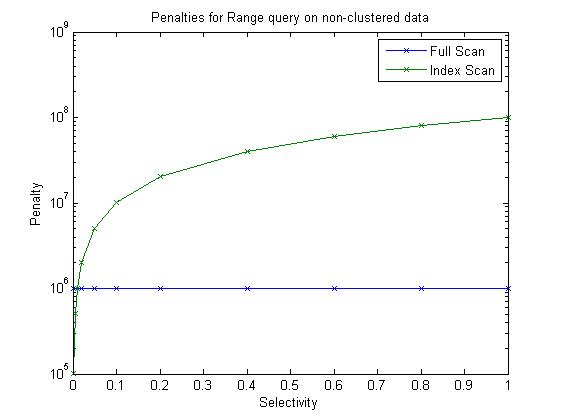
\includegraphics[width=0.45\textwidth]{images/Result2-Factor10}
	\label{fig:subfig1.1}}
\quad
\subfigure[Factor 20]{%
	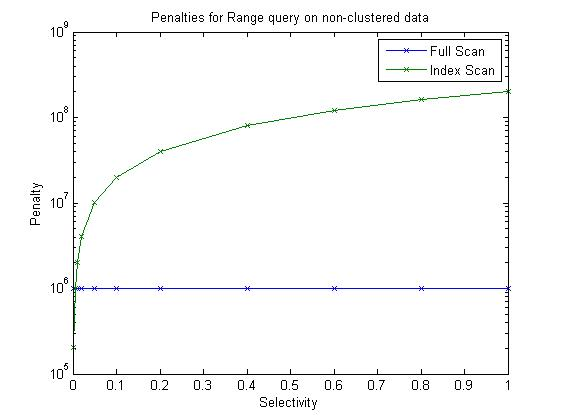
\includegraphics[width=0.45\textwidth]{images/Result1-Factor20}
	\label{fig:subfig1.2}}

\subfigure[Factor 50]{%
	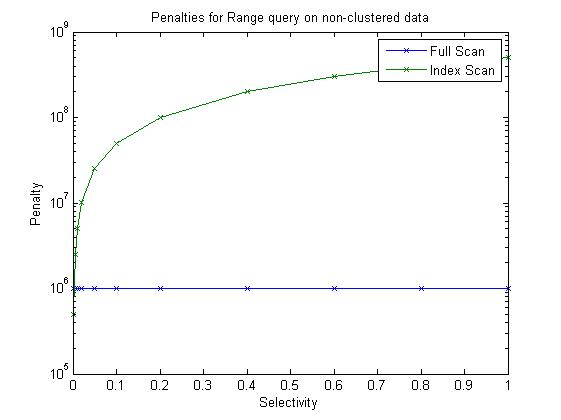
\includegraphics[width=0.45\textwidth]{images/Result3-Factor50}
	\label{fig:subfig1.3}}
\quad
\subfigure[Factor 100]{%
	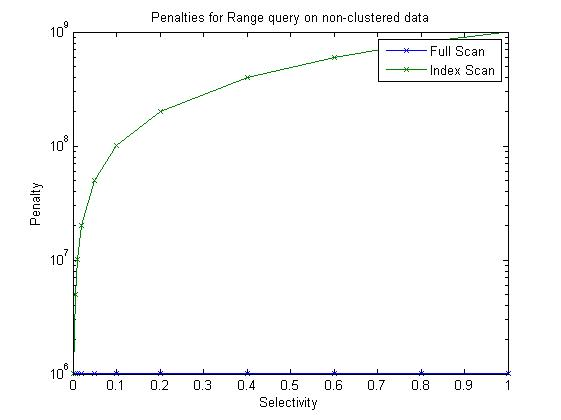
\includegraphics[width=0.45\textwidth]{images/Result4-Factor100}
	\label{fig:subfig1.4}}
%	
\label{fig:result1}
\caption{Penalties for index scan and full scan for a random query}
\end{figure}
\pagebreak


\section{Progress}
So far, we have created several scripts in Matlab that should simulate the real performances of the several scans. However the results of our Matlab scripts do not completely match with the results we see in the actual report, for example: in our report the full scan performs better for selectivity $>$ 0.005, while in \cite{smoothscan} this only holds for selectivity $>$ 0.15. Because of these differences we have our doubts concerning the simulations we made, we want to verify the assumptions we made and check our code for any errors we might have made.

Since the editors of \cite{smoothscan} would not give us the code used in their article, we plan to keep on simulating the several scanning algorithms rather then performing actual read/write actions on hard drives. Matlab allows us to quickly create a simulation and output it to a graph, which is very convenient and quicker than using an actual programming language such as Java. Because of this we are planning to keep on using Matlab and we will not use actual read/write actions on hard drives.

\section{Conclusion}
todo

\begin{thebibliography}{9}

\bibitem{smoothscan}
	 Borovica, R., Idreos, S., Ailamaki, A., Zukowski, M., $\&$ Fraser, C.
	2015.	
 	Smooth Scan: One access path to rule them all.
	\emph{IEEE International conference on Data Engineering.}

\bibitem{query}
	Deshpande, A., Ives, Z., $\&$ Raman, V.
	2007.
	Adaptive query processing
	\emph{Foundations and Trends in Databases,}
	1(1), 1-140.
\end{thebibliography}
\newpage

\begin{appendices}
\section{Code index scan}
\label{appendixa}
\lstinputlisting{Simulation/IndexScan.m}
\section{Code full scan}
\label{appendixb}
\lstinputlisting{Simulation/FullScan.m}
\section{Code switch scan}
\label{appendixb}
\lstinputlisting{Simulation/SwitchScan.m}
\end{appendices}

\end{document}
